\documentclass{beamer}
\usepackage[utf8]{inputenc}
\usepackage[]{amsmath}
\usepackage{graphicx}
\usepackage{physics}
\usepackage{subcaption} % package pour faire des subfigures
\usepackage{multirow} % package pour multirow/multicolumn
\usepackage{booktabs} % package pour top/mid/bottom rule
\usepackage{tcolorbox} % toujours plus de boites
%\usepackage[backend=biber]{biblatex}
%
%
%\addbibresource{Biblio_dbl_quantum.bib}

%\bibliographystyle{stylename}
%\bibliography{Biblio_dbl_quantum}

\title{Low field depolarization of dense NV centers ensemble: application to magnetometry}
\author{Clément Pellet-Mary, Maxime Perdriat, Paul Huillery,\\ Gabriel Hétet}
\date{Nano-optics group}

\mode<presentation> {\usetheme{Rochester}}

\begin{document}
\begin{frame}
\maketitle
\begin{center}
\includegraphics[width=\textwidth,height=0.3\textheight,keepaspectratio]{logos}
\end{center}
\end{frame}
%\begin{frame}{Outline}
%\tableofcontents
%\end{frame}
%\section{Physics of the NV center}
\begin{frame}{Preamble : the NV center}
\centering
\includegraphics[width=\textwidth,height=0.9\textheight,keepaspectratio]{Slide  NV properties}
\end{frame}

\begin{frame}{Preamble : the 4 classes of NV centers}
\centering
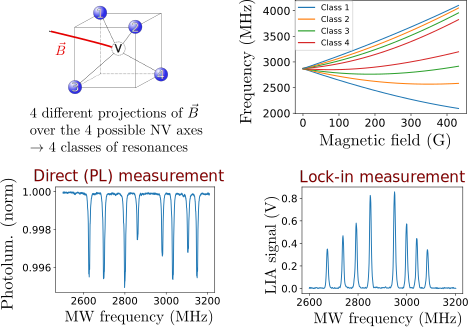
\includegraphics[width=\textwidth,height=0.9\textheight,keepaspectratio]{slide ODMR 4 classes}
\end{frame}

\begin{frame}{Subject of this presentation}
\centering
\includegraphics[width=\textwidth,height=0.9\textheight,keepaspectratio]{slide_presentation_sujet}
\end{frame}

\begin{frame}{Outline}
\tableofcontents
\end{frame}



\section{Cross-relaxation with NV centers}
\begin{frame}{Outline}
\tableofcontents[currentsection]
\end{frame}
\begin{frame}{Principle of cross-relaxation with NV centers}
\centering
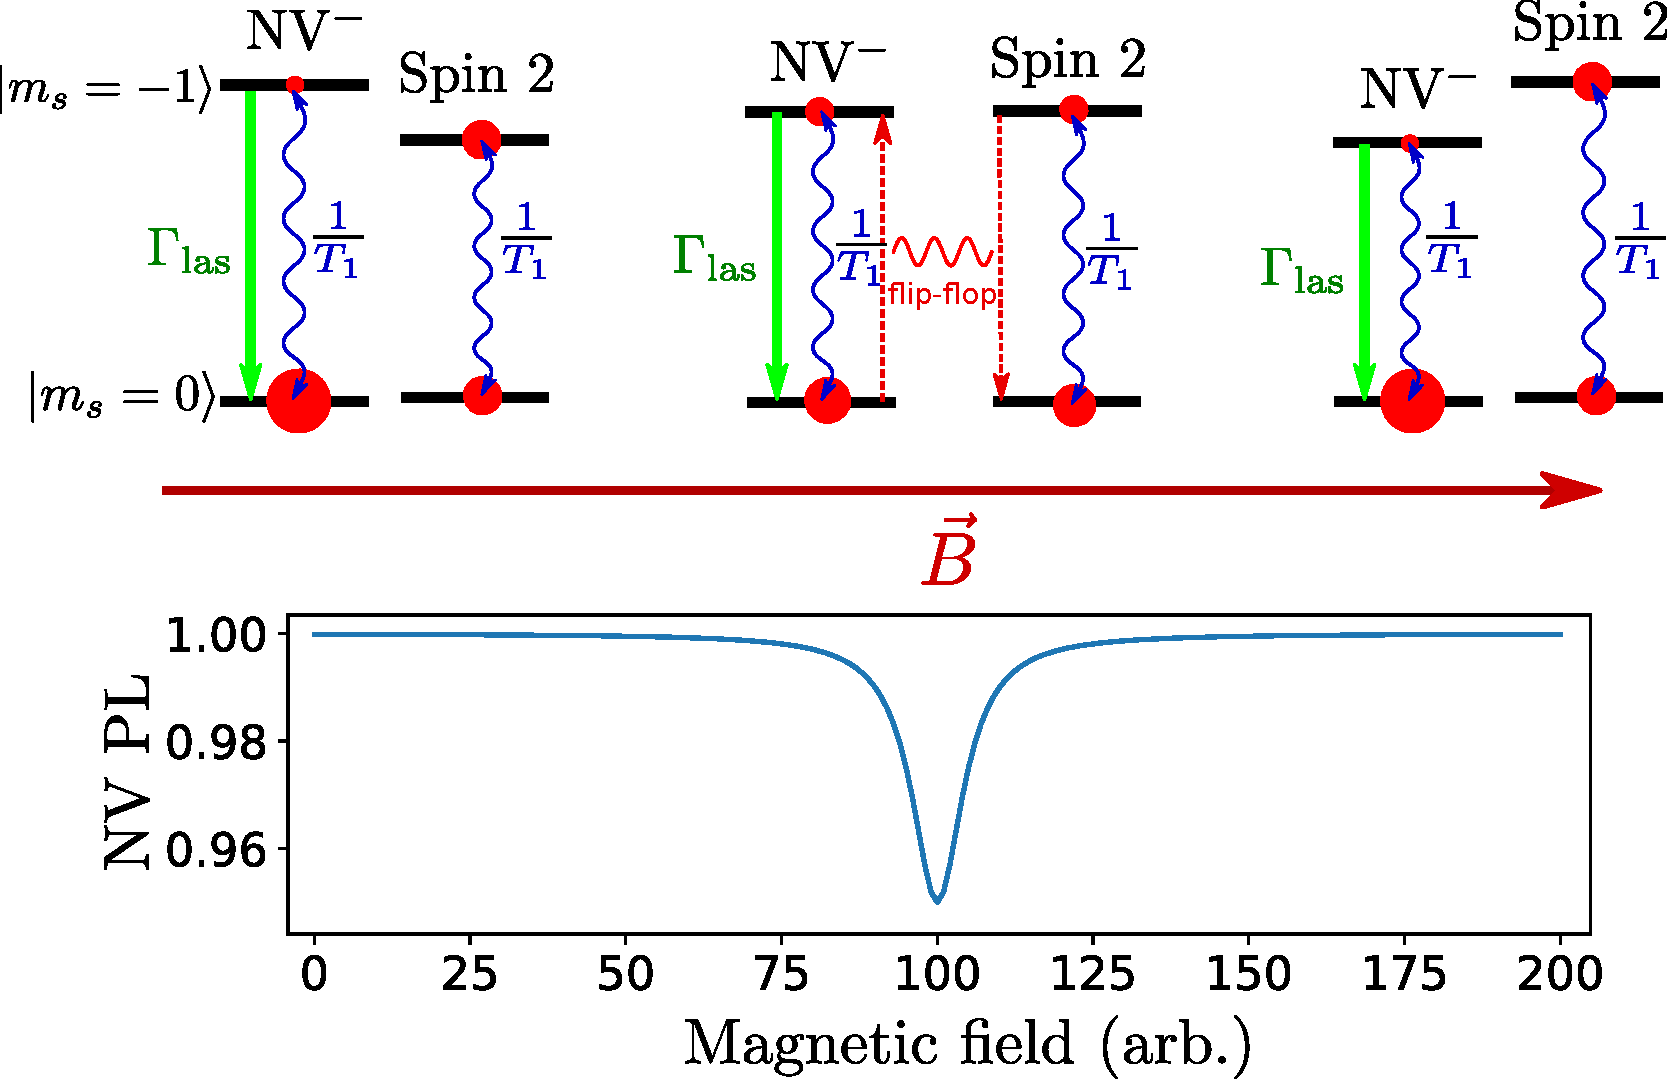
\includegraphics[width=\textwidth,height=0.8\textheight,keepaspectratio]{Slide_CR_presentation}
\end{frame}

\begin{frame}{Example: Cross-relaxation between NV centers and VH$^-$}
\centering
\includegraphics[width=\textwidth,height=0.9\textheight,keepaspectratio]{Slide_CR_VH}
\end{frame}

\begin{frame}{Cross-relaxation between NV centers and NV centers}
\centering
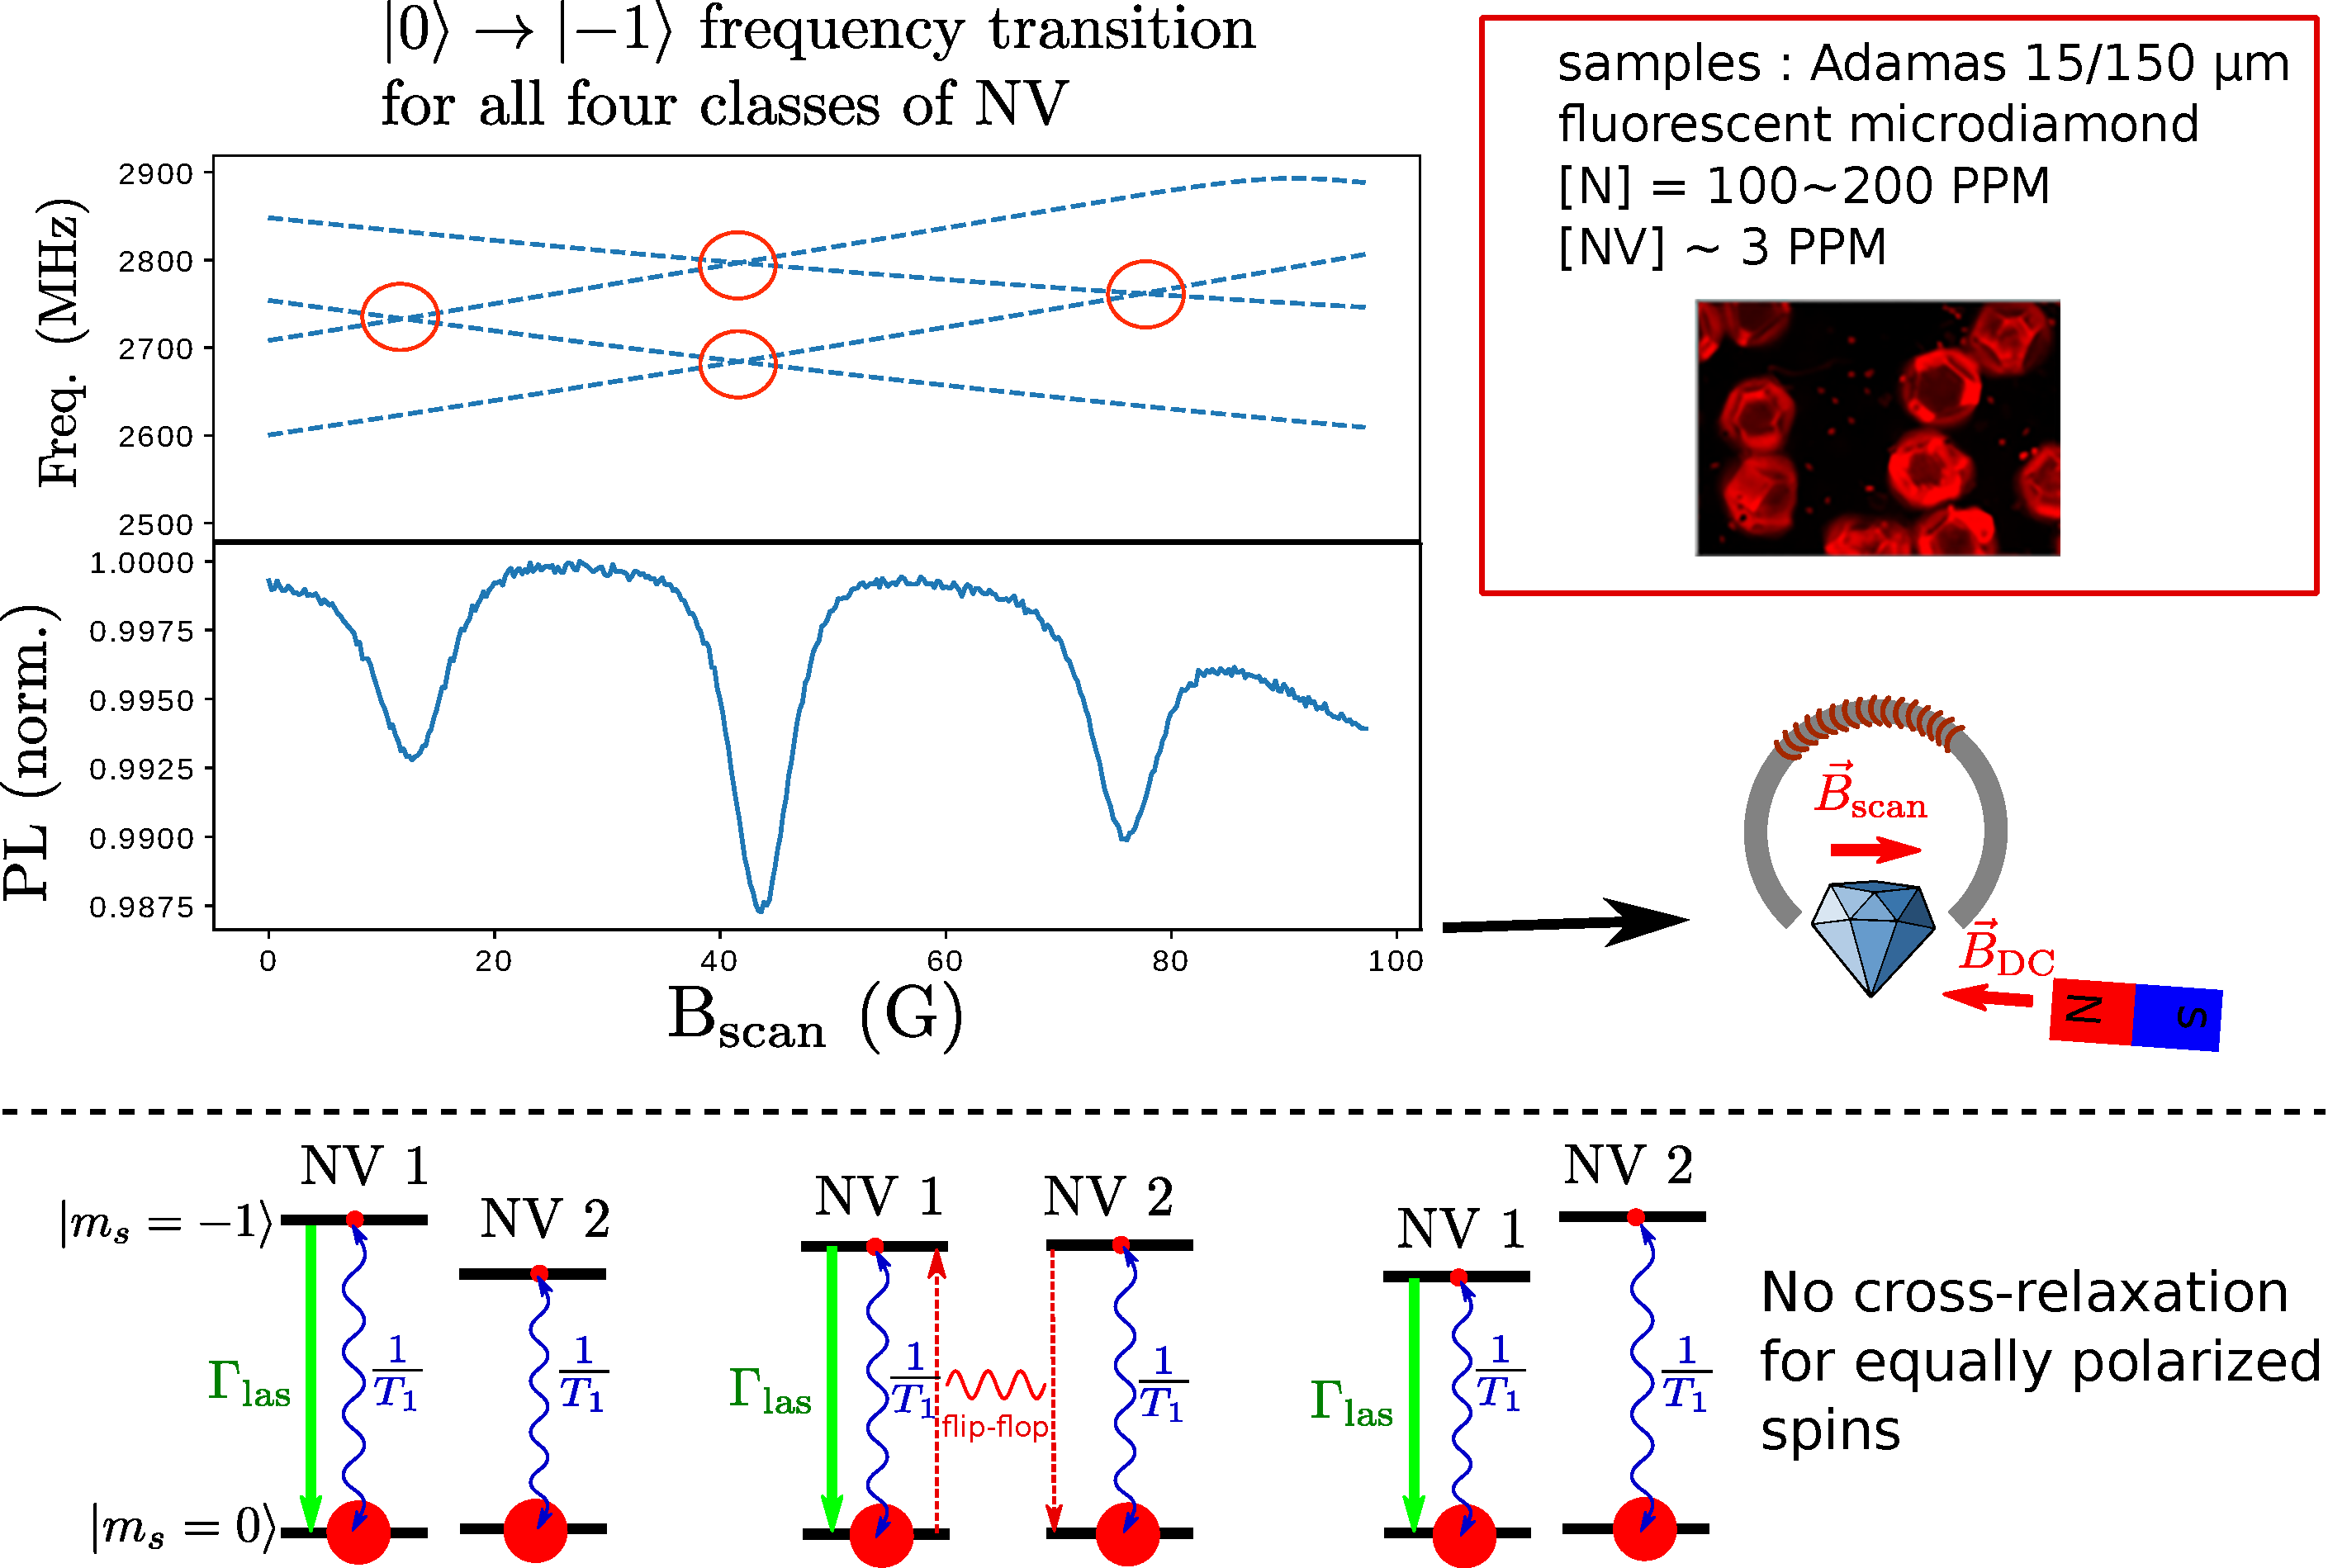
\includegraphics[width=\textwidth,height=0.9\textheight,keepaspectratio]{Slide_CR_adamas}
\end{frame}
\section{The NV-fluctuator model and experimental verification}
\begin{frame}{Outline}
\tableofcontents[currentsection]
\end{frame}
\begin{frame}{Presentation of the fluctuator model}
\centering
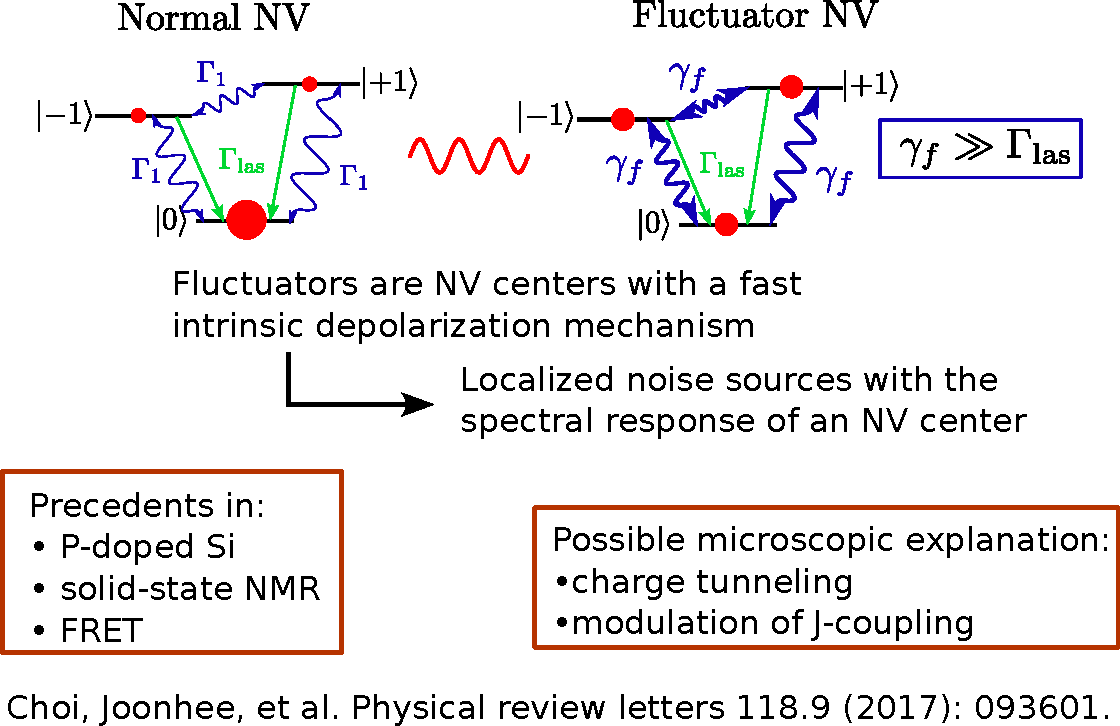
\includegraphics[width=\textwidth,height=0.8\textheight,keepaspectratio]{Slide_fluct_intro}
\end{frame}

\begin{frame}{Predictions of the fluctuator model}
\begin{itemize}
\item $\Gamma_1$ increases when classes overlap spectrally (increase in the resonant fluctuator density).
\item The dipole induced depolarization has a stretched exponential profile:
$$ \rho_{00}(t) \propto \exp(-\sqrt{\frac{t}{T_1}})$$
\item The Fluctuators spectral response is broadened by their decay rate $\gamma_f$ (lifetime limit).
\end{itemize}
\end{frame}

\begin{frame}{$T_1$ measurement protocol}
\centering
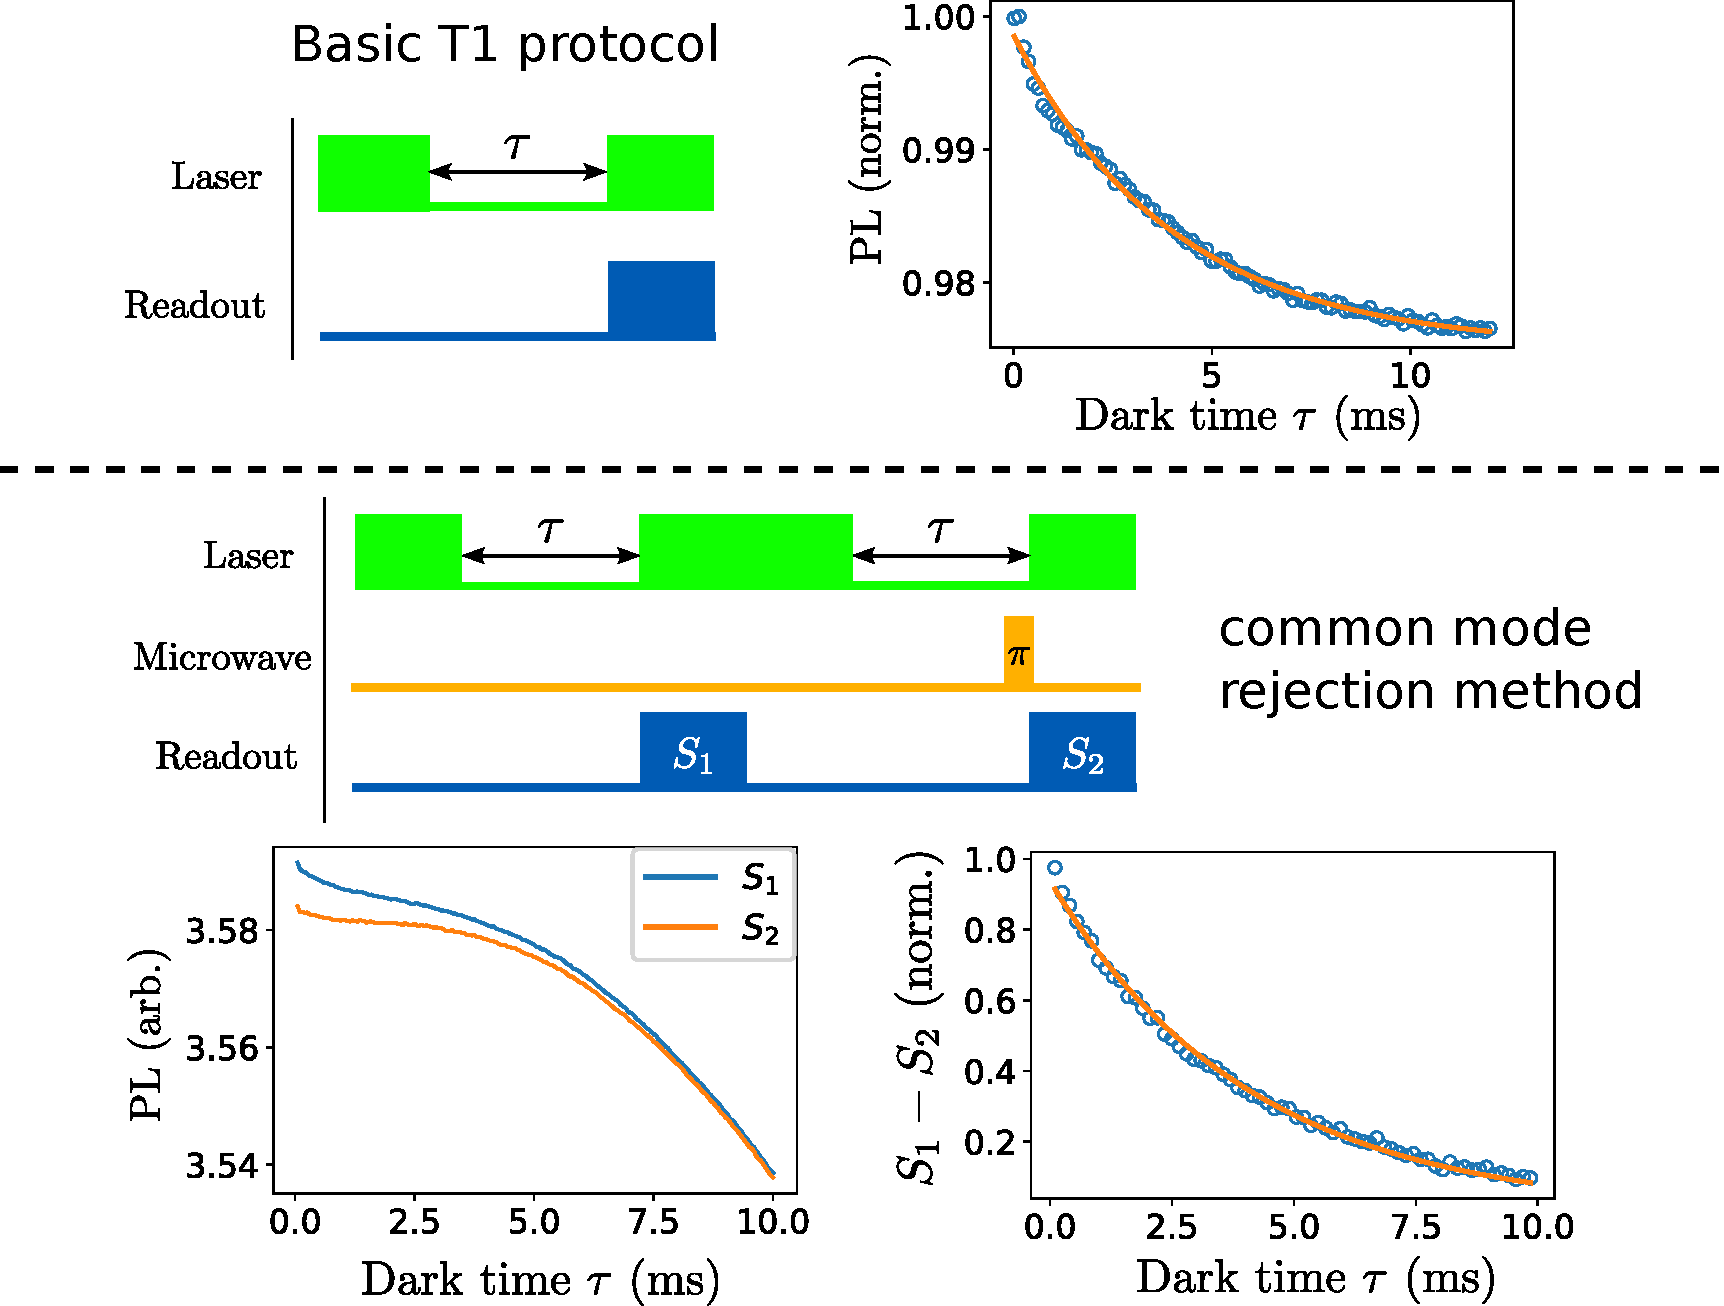
\includegraphics[width=\textwidth,height=0.9\textheight,keepaspectratio]{slide_T1_protocol}
\end{frame}

\begin{frame}{Stretched exponential decay profile}
\centering
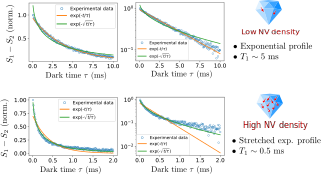
\includegraphics[width=\textwidth,height=0.9\textheight,keepaspectratio]{Slide_T1_exp_stretch}
\end{frame}

\begin{frame}{Competition between stretched and exponential decay}
\centering
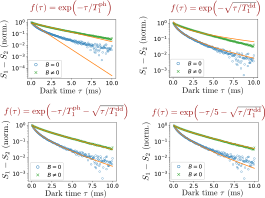
\includegraphics[width=\textwidth,height=0.9\textheight,keepaspectratio]{Slide_T1_exp_et_stretch}
\end{frame}

\begin{frame}{Spectral response of the fluctuators}
\centering
\includegraphics[width=\textwidth,height=0.9\textheight,keepaspectratio]{Slide_fluct_linewidth}
\end{frame}

\begin{frame}{Geometry conditions for class resonances}
\centering
\includegraphics[width=\textwidth,height=0.9\textheight,keepaspectratio]{Slide_geométries}
\end{frame}

\begin{frame}{PL mapping of the crystalline planes}
\centering
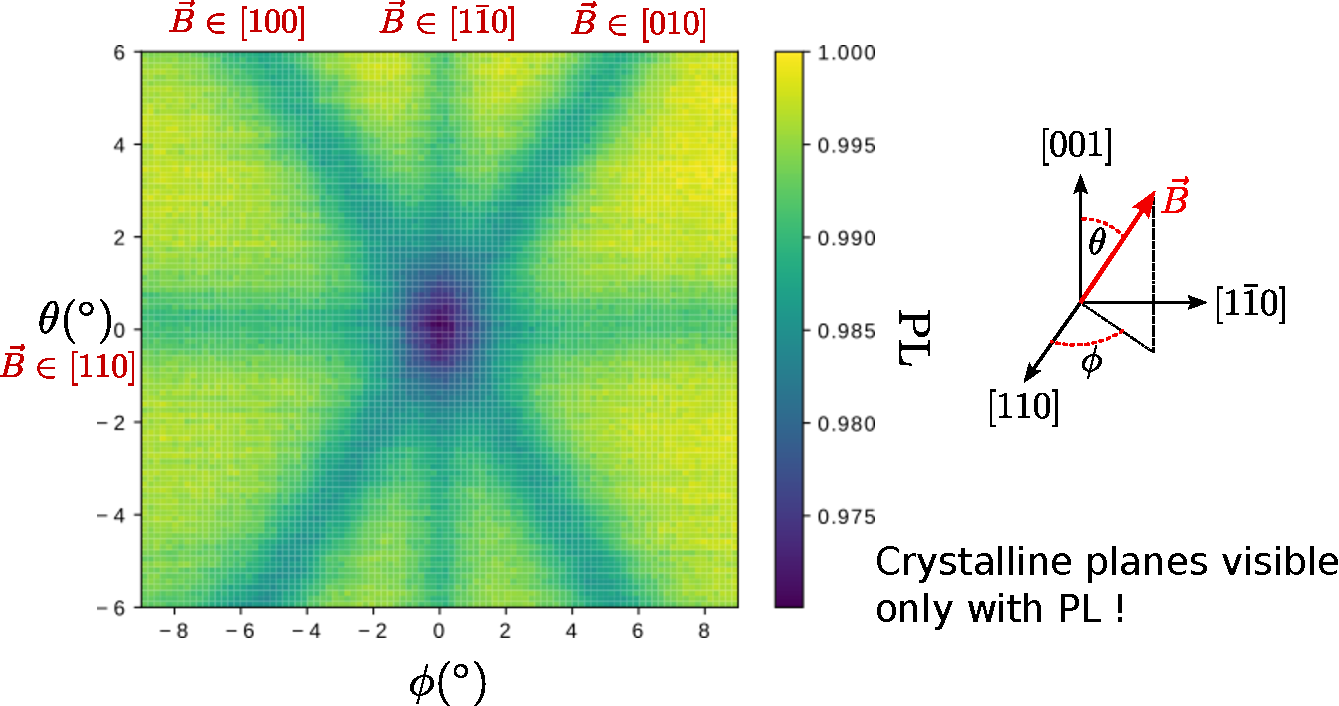
\includegraphics[width=\textwidth,height=0.8\textheight,keepaspectratio]{Slide_carte}
\end{frame}

\begin{frame}{Limitations of the fluctuator model}
\centering
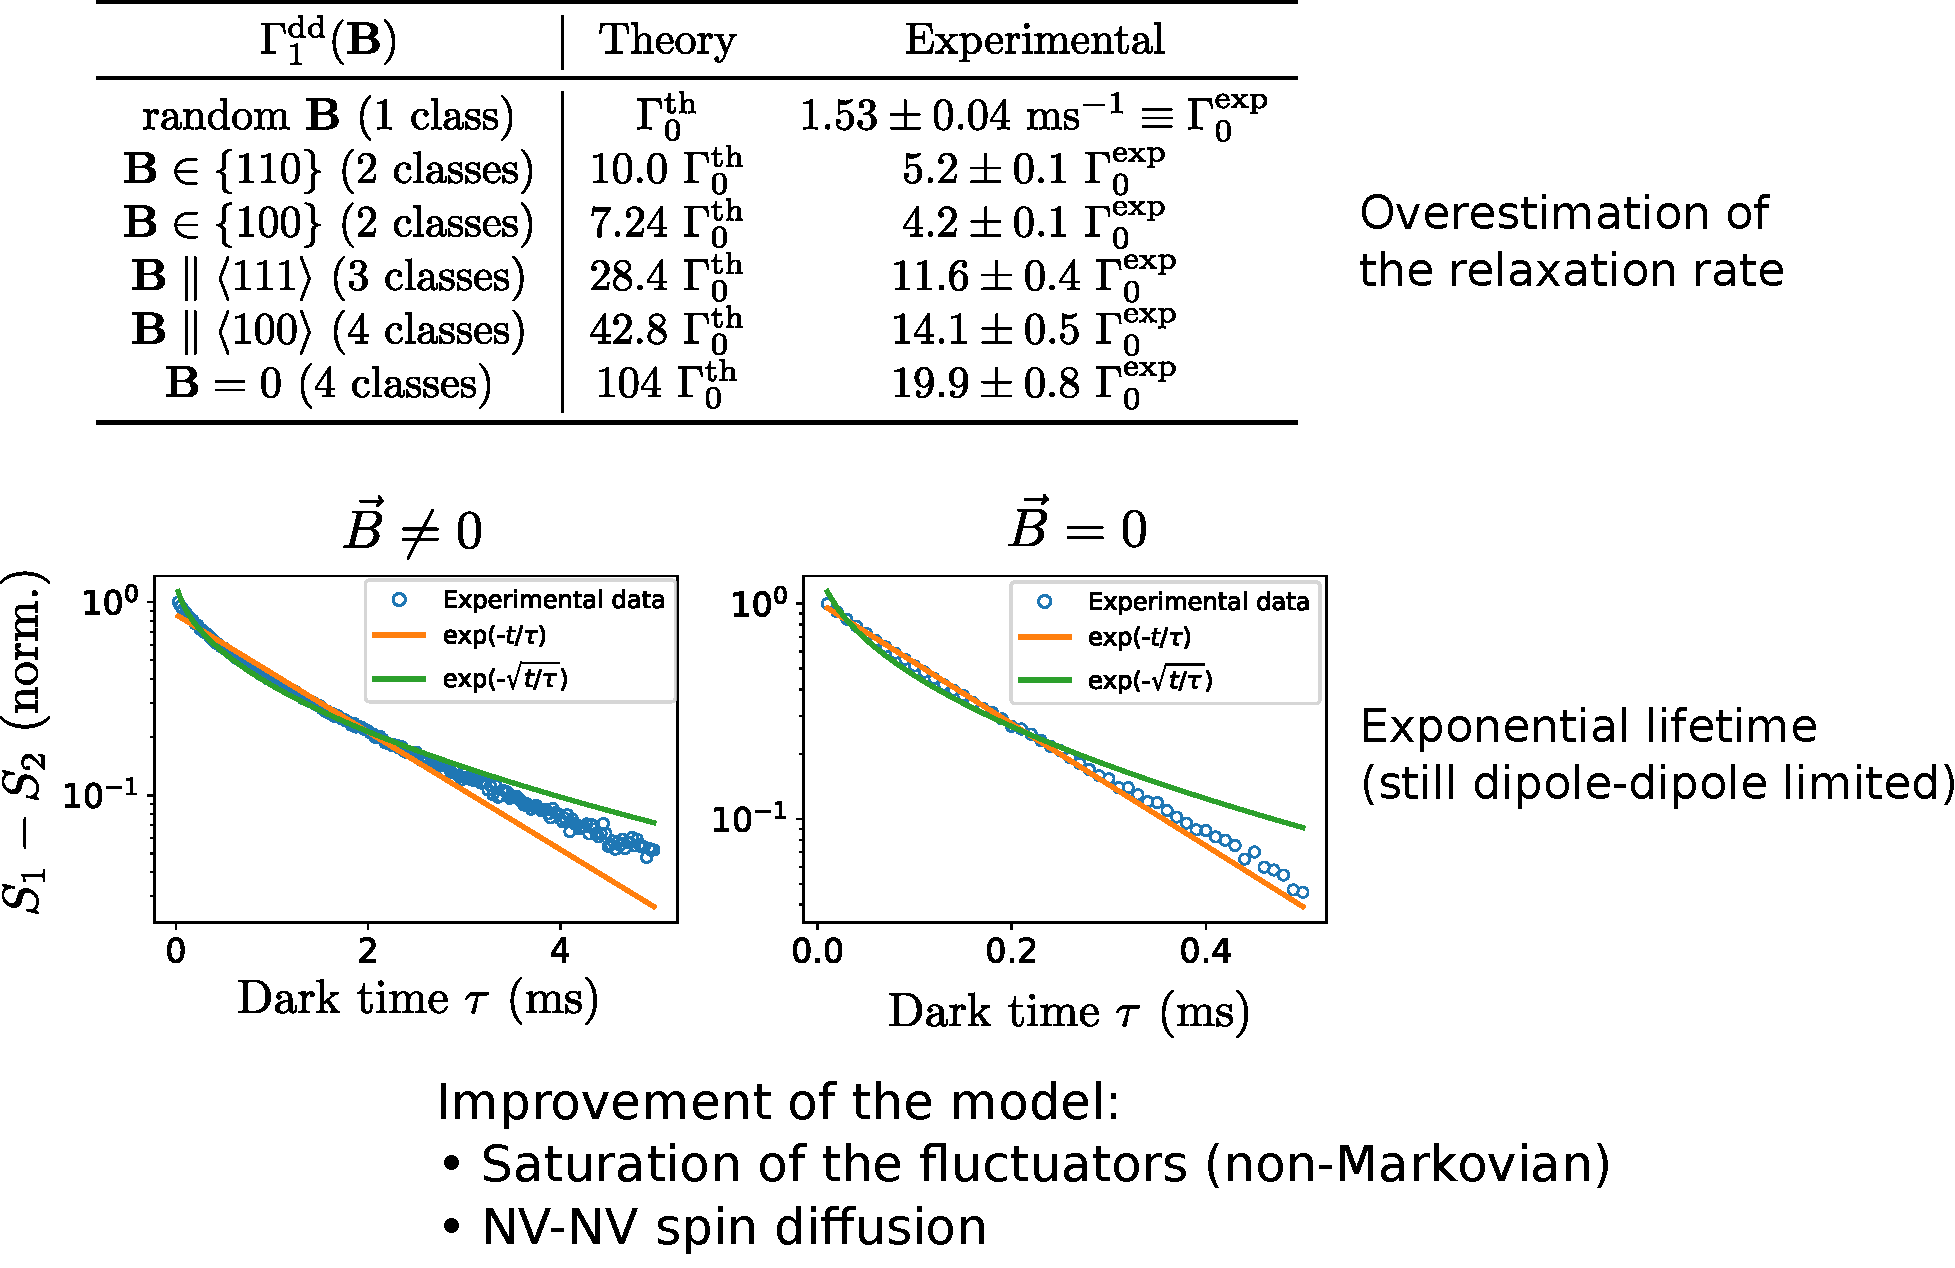
\includegraphics[width=\textwidth,height=0.9\textheight,keepaspectratio]{Slide_limit_fluct}
\end{frame}

\section{Dipole-dipole interaction under low magnetic field}
\begin{frame}{Outline}
\tableofcontents[currentsection]
\end{frame}
\begin{frame}{Zero field depolarization sources (theory)}
\centering
\includegraphics[width=\textwidth,height=0.9\textheight,keepaspectratio]{Slide_0B_theorie}
\end{frame}

\begin{frame}{Experiment: $\vec B$ in arbitrary direction}
\centering
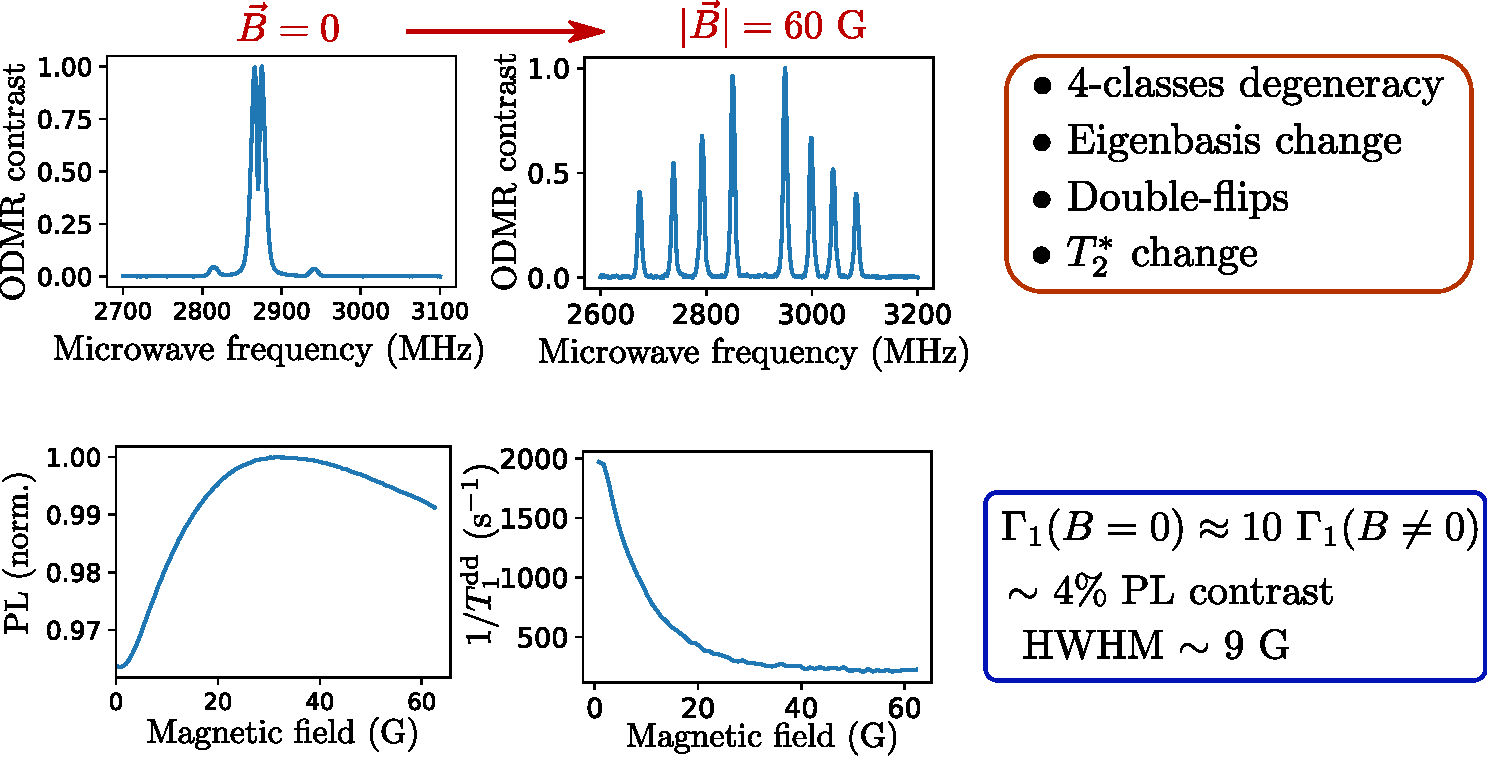
\includegraphics[width=\textwidth,height=0.9\textheight,keepaspectratio]{Slide_T1_PL_1x1x1x1}
\end{frame}

\begin{frame}{Experiment: $\vec B \parallel [100]$}
\centering
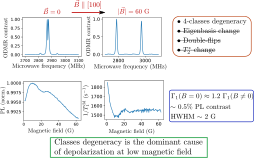
\includegraphics[width=\textwidth,height=0.9\textheight,keepaspectratio]{Slide_T1_PL_100}
\end{frame}

\begin{frame}{Experiment: $\vec B \perp [111]$}
\centering
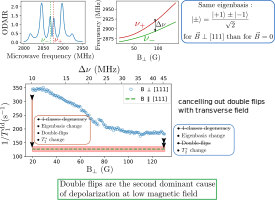
\includegraphics[width=\textwidth,height=0.9\textheight,keepaspectratio]{slide_champs_transverse}
\end{frame}

\begin{frame}{Summary of the experimental observations}
\centering
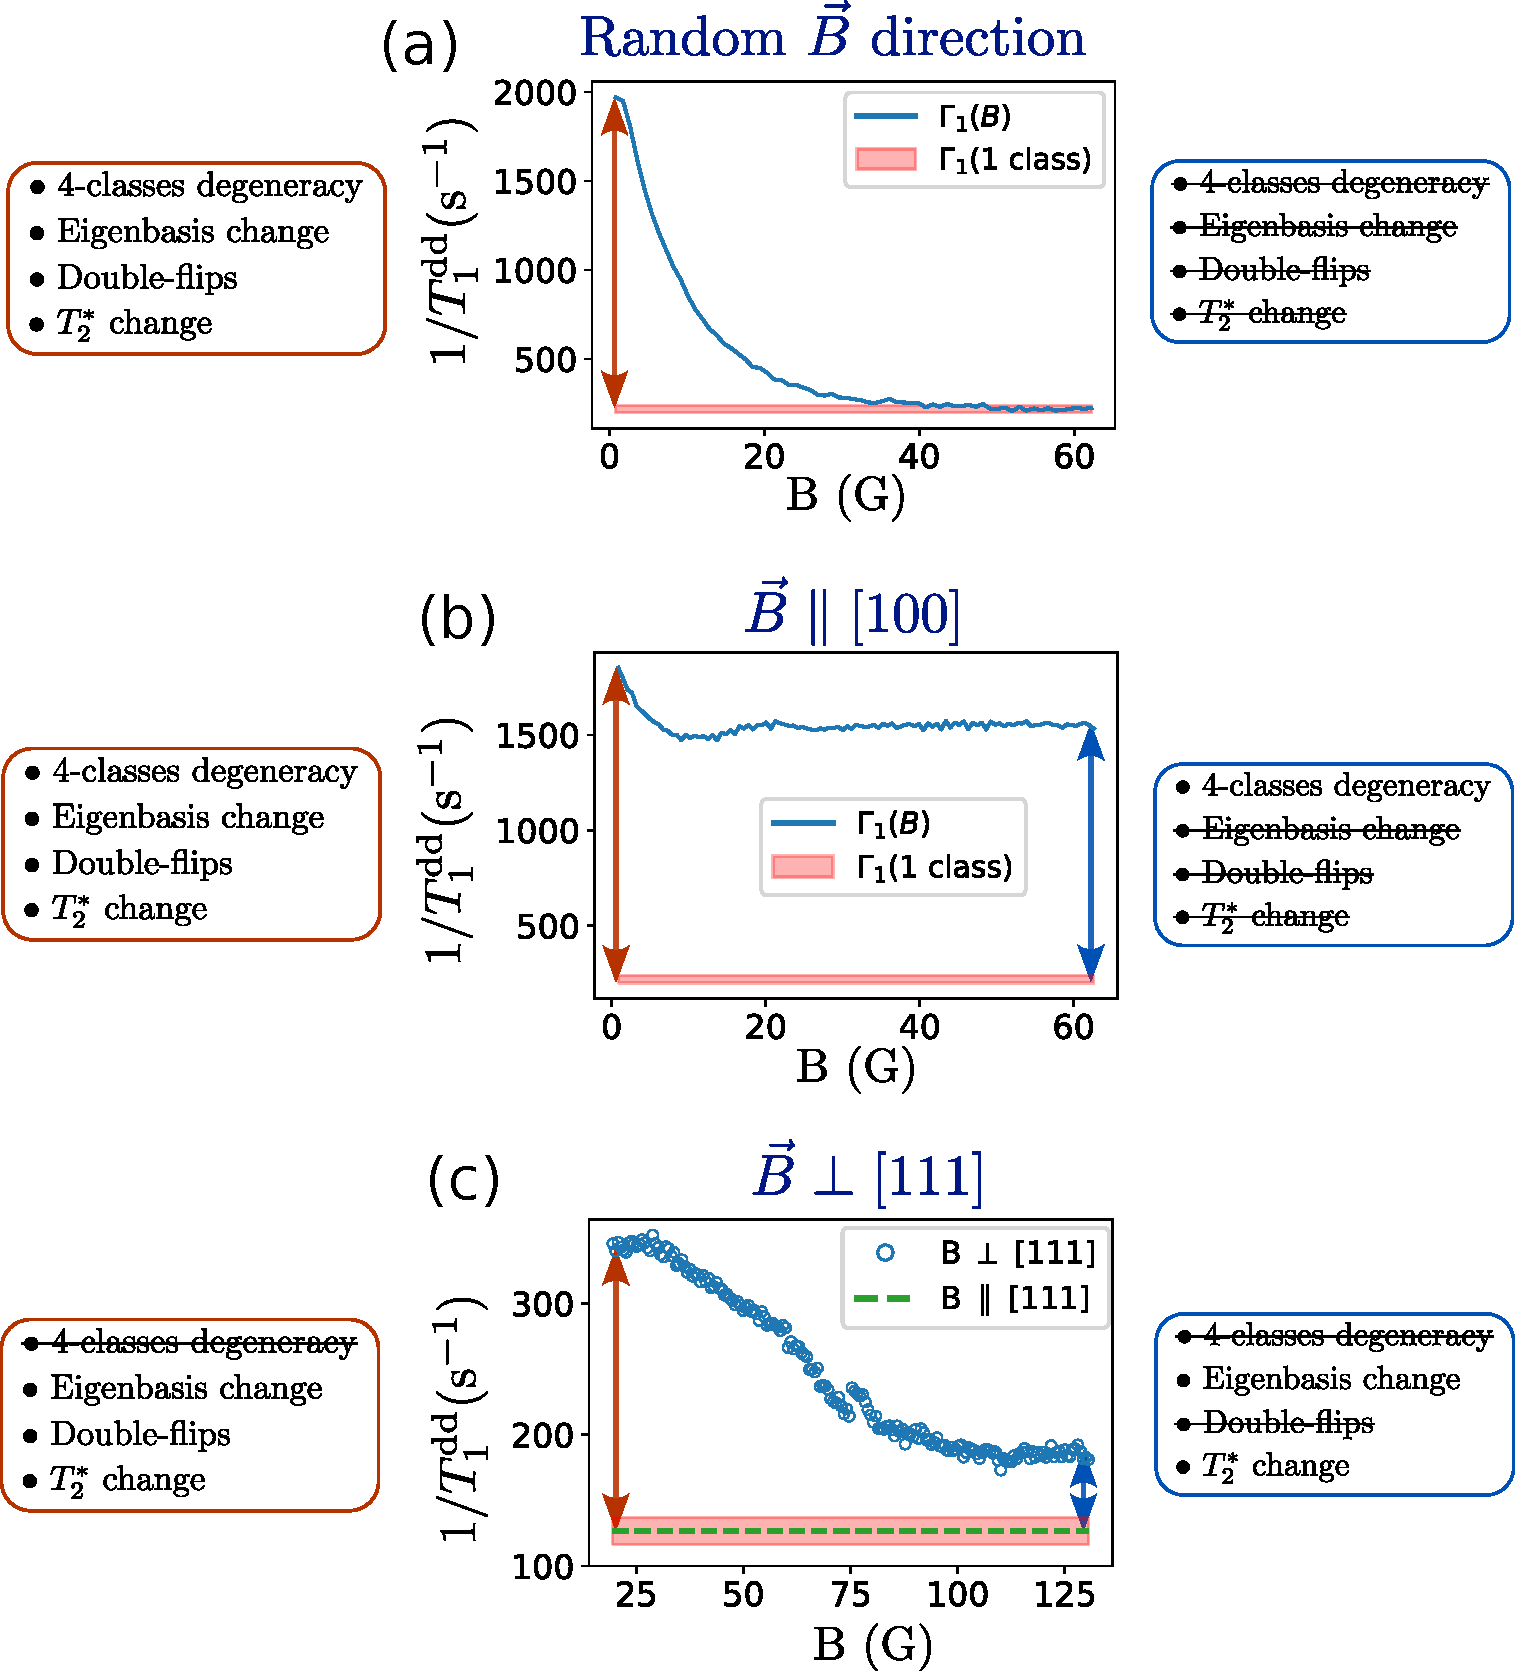
\includegraphics[width=\textwidth,height=0.9\textheight,keepaspectratio]{shema_summary_exp}
\end{frame}

\section{Low field depolarization magnetometry (LFDM)}
\begin{frame}{Outline}
\tableofcontents[currentsection]
\end{frame}
\begin{frame}{Principle of LFDM}
\centering
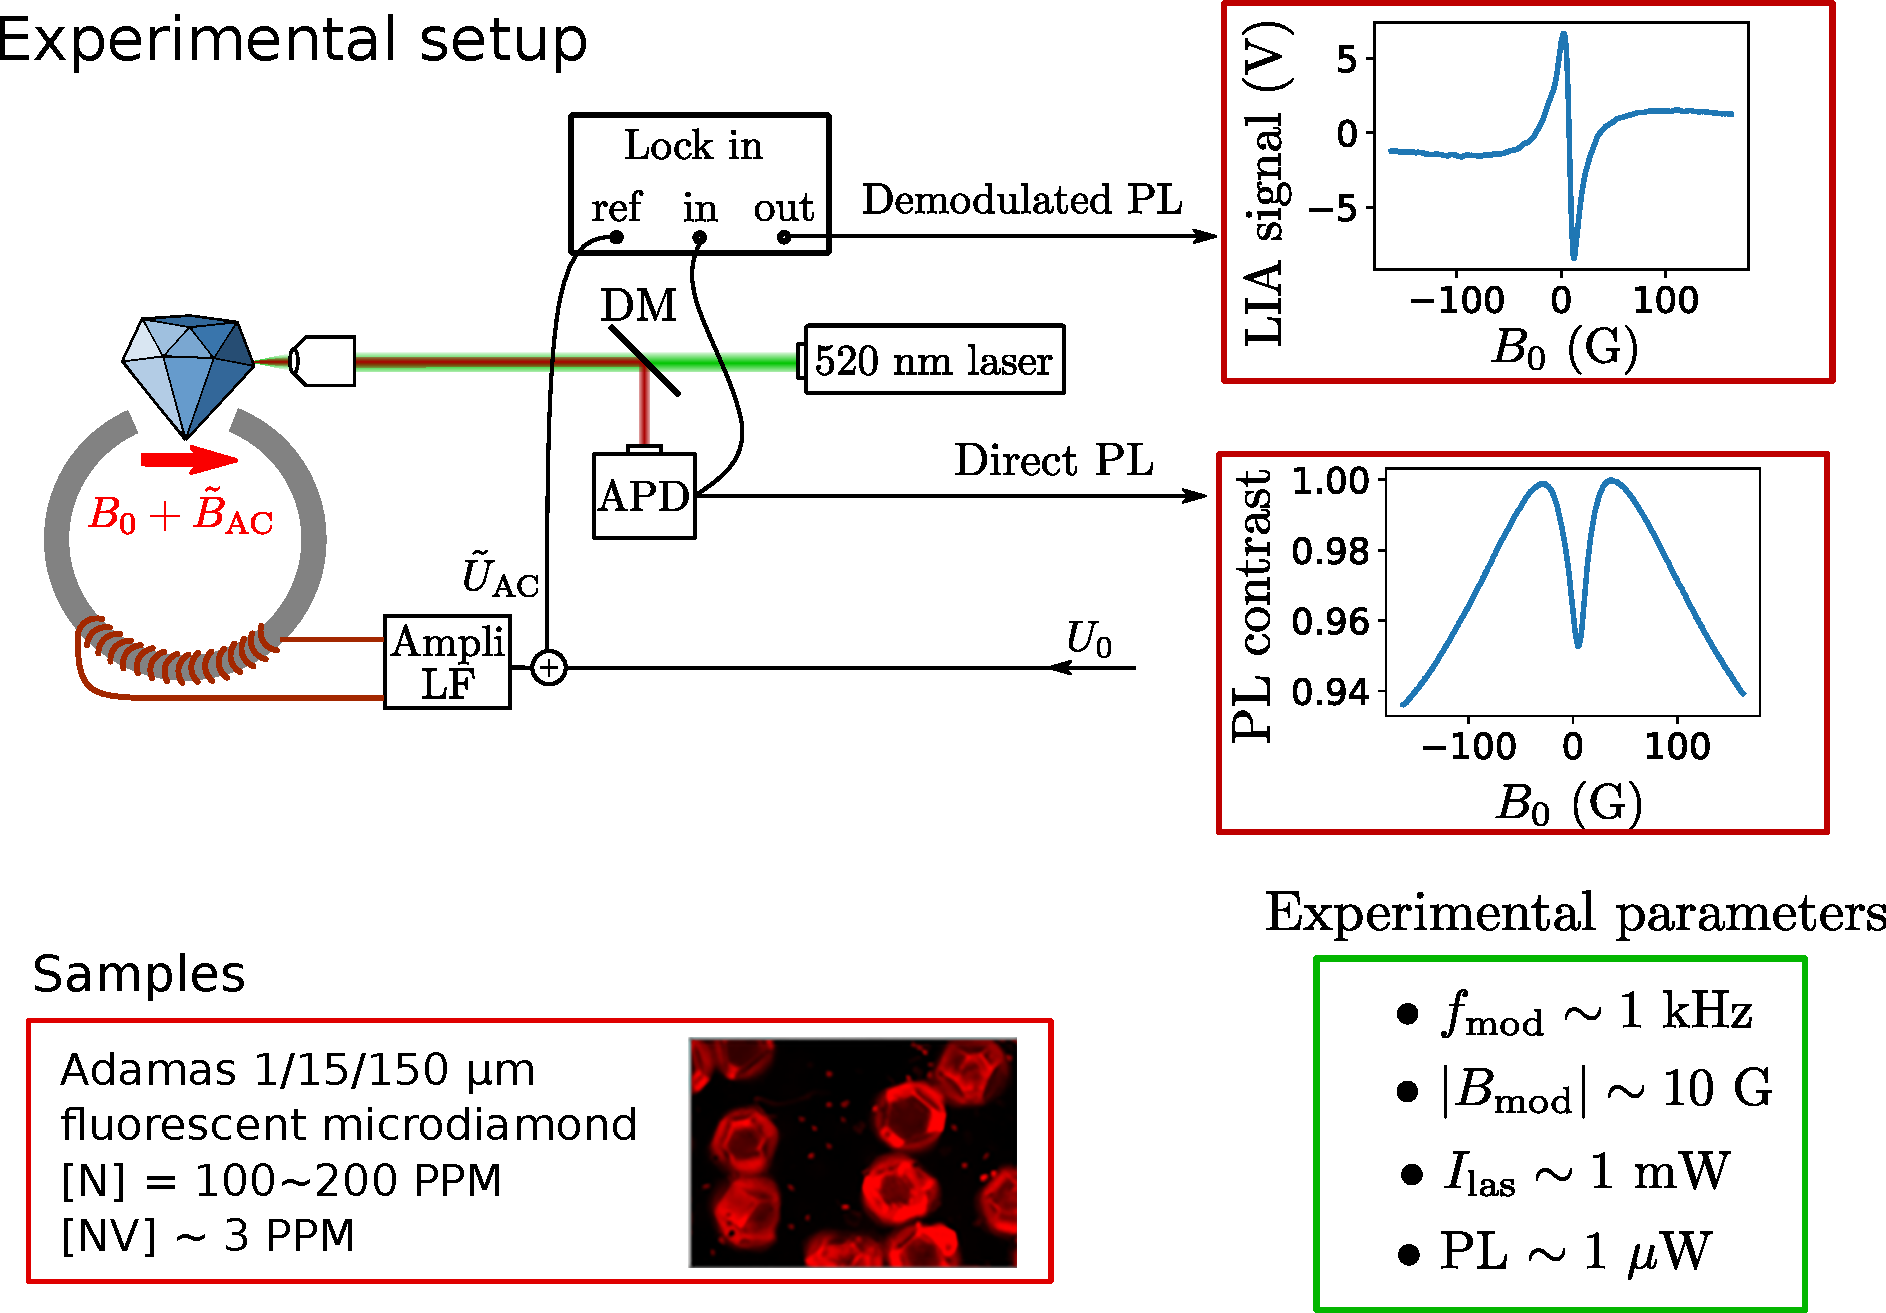
\includegraphics[width=\textwidth,height=0.9\textheight,keepaspectratio]{Slide_principle_LFDM}
\end{frame}

\begin{frame}{Sensitivity of LFDM}
\centering
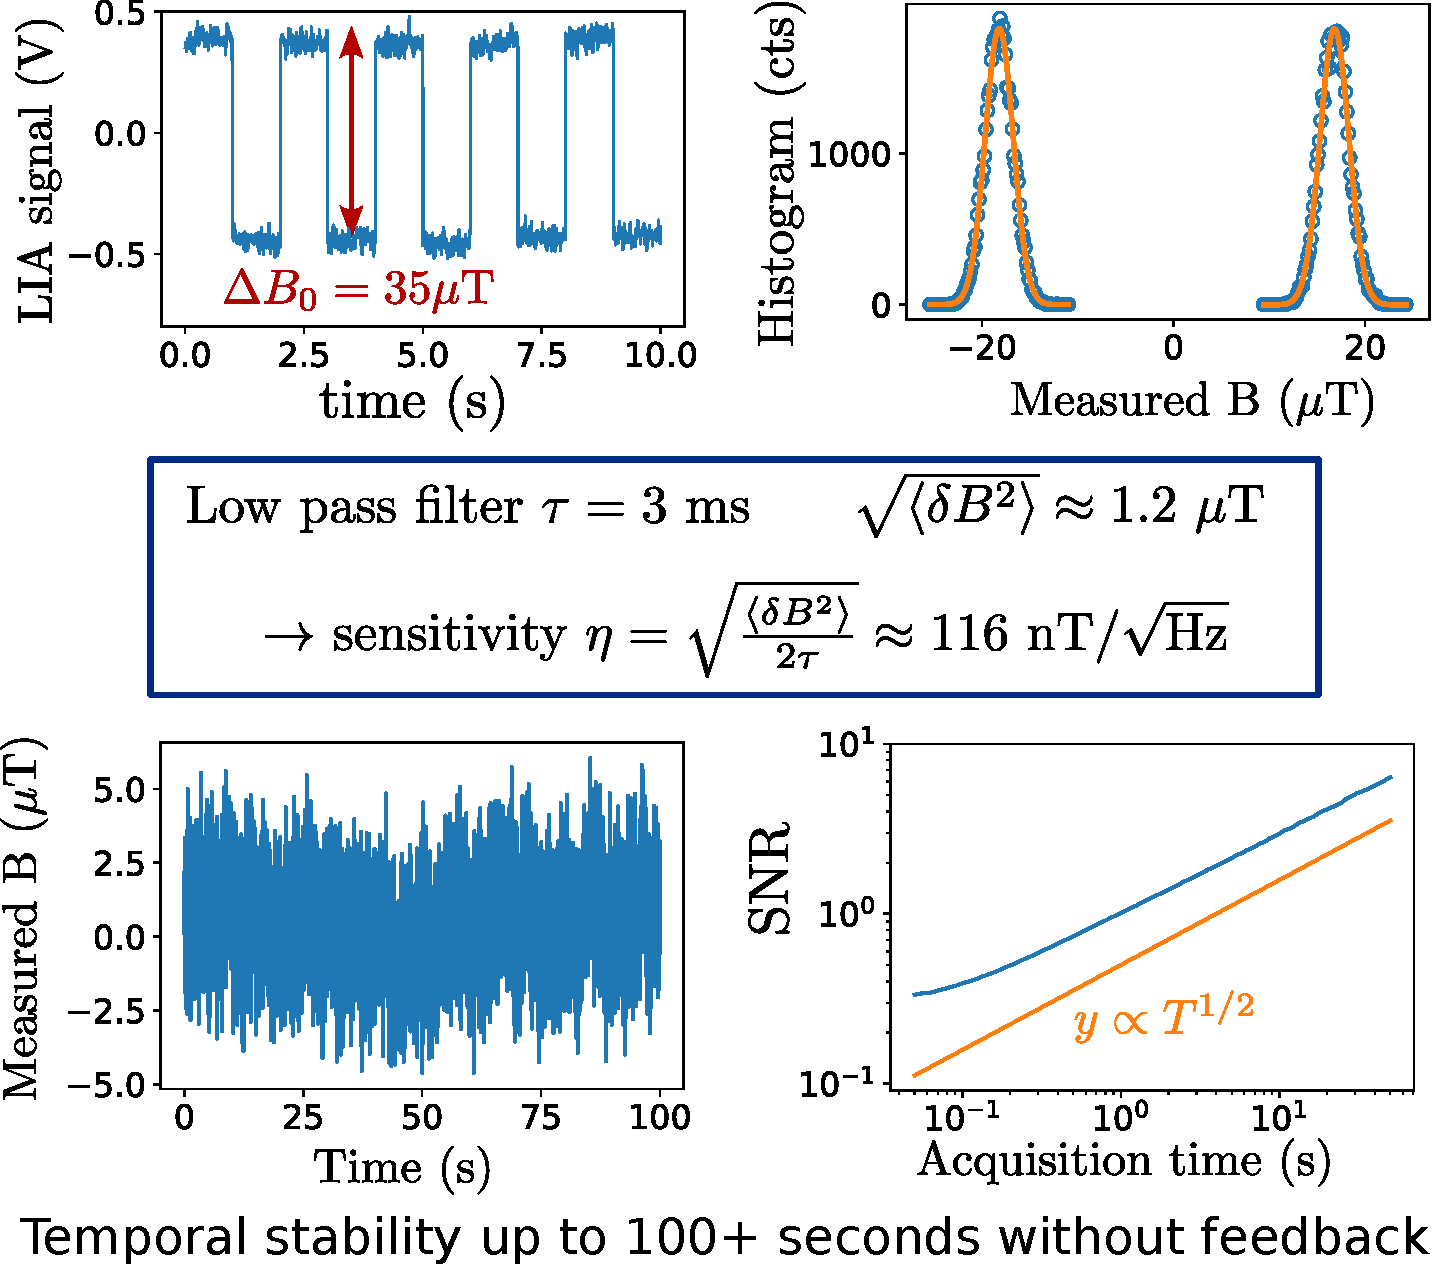
\includegraphics[width=\textwidth,height=0.9\textheight,keepaspectratio]{Slide_sensi_LFDM}
\end{frame}

\begin{frame}{Comparison with the state of the art}
\centering
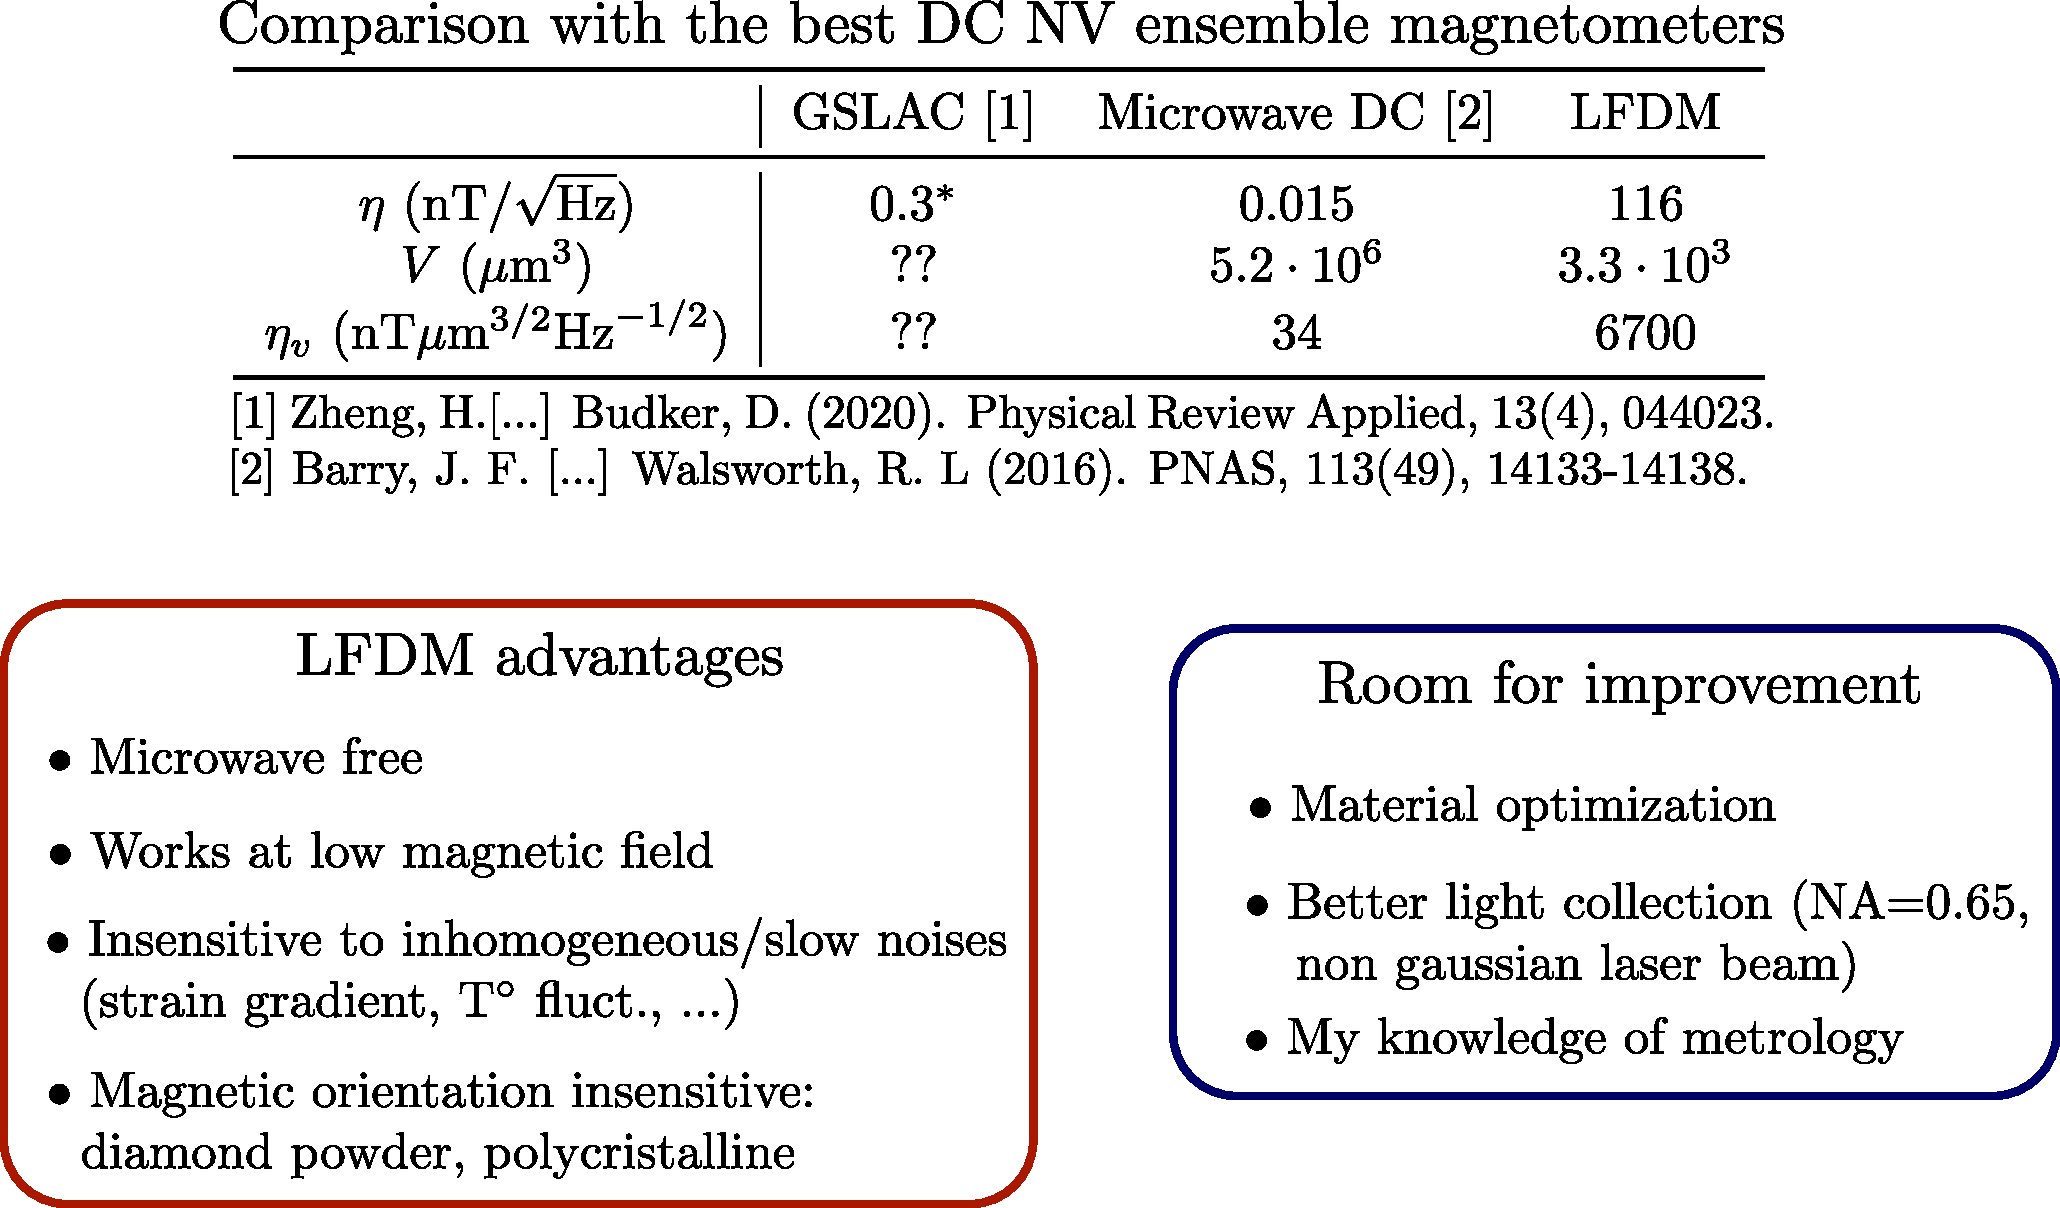
\includegraphics[width=\textwidth,height=0.9\textheight,keepaspectratio]{Slide_comparison_litterature}
\end{frame}

\begin{frame}{Comparison with CW ODMR}
\centering
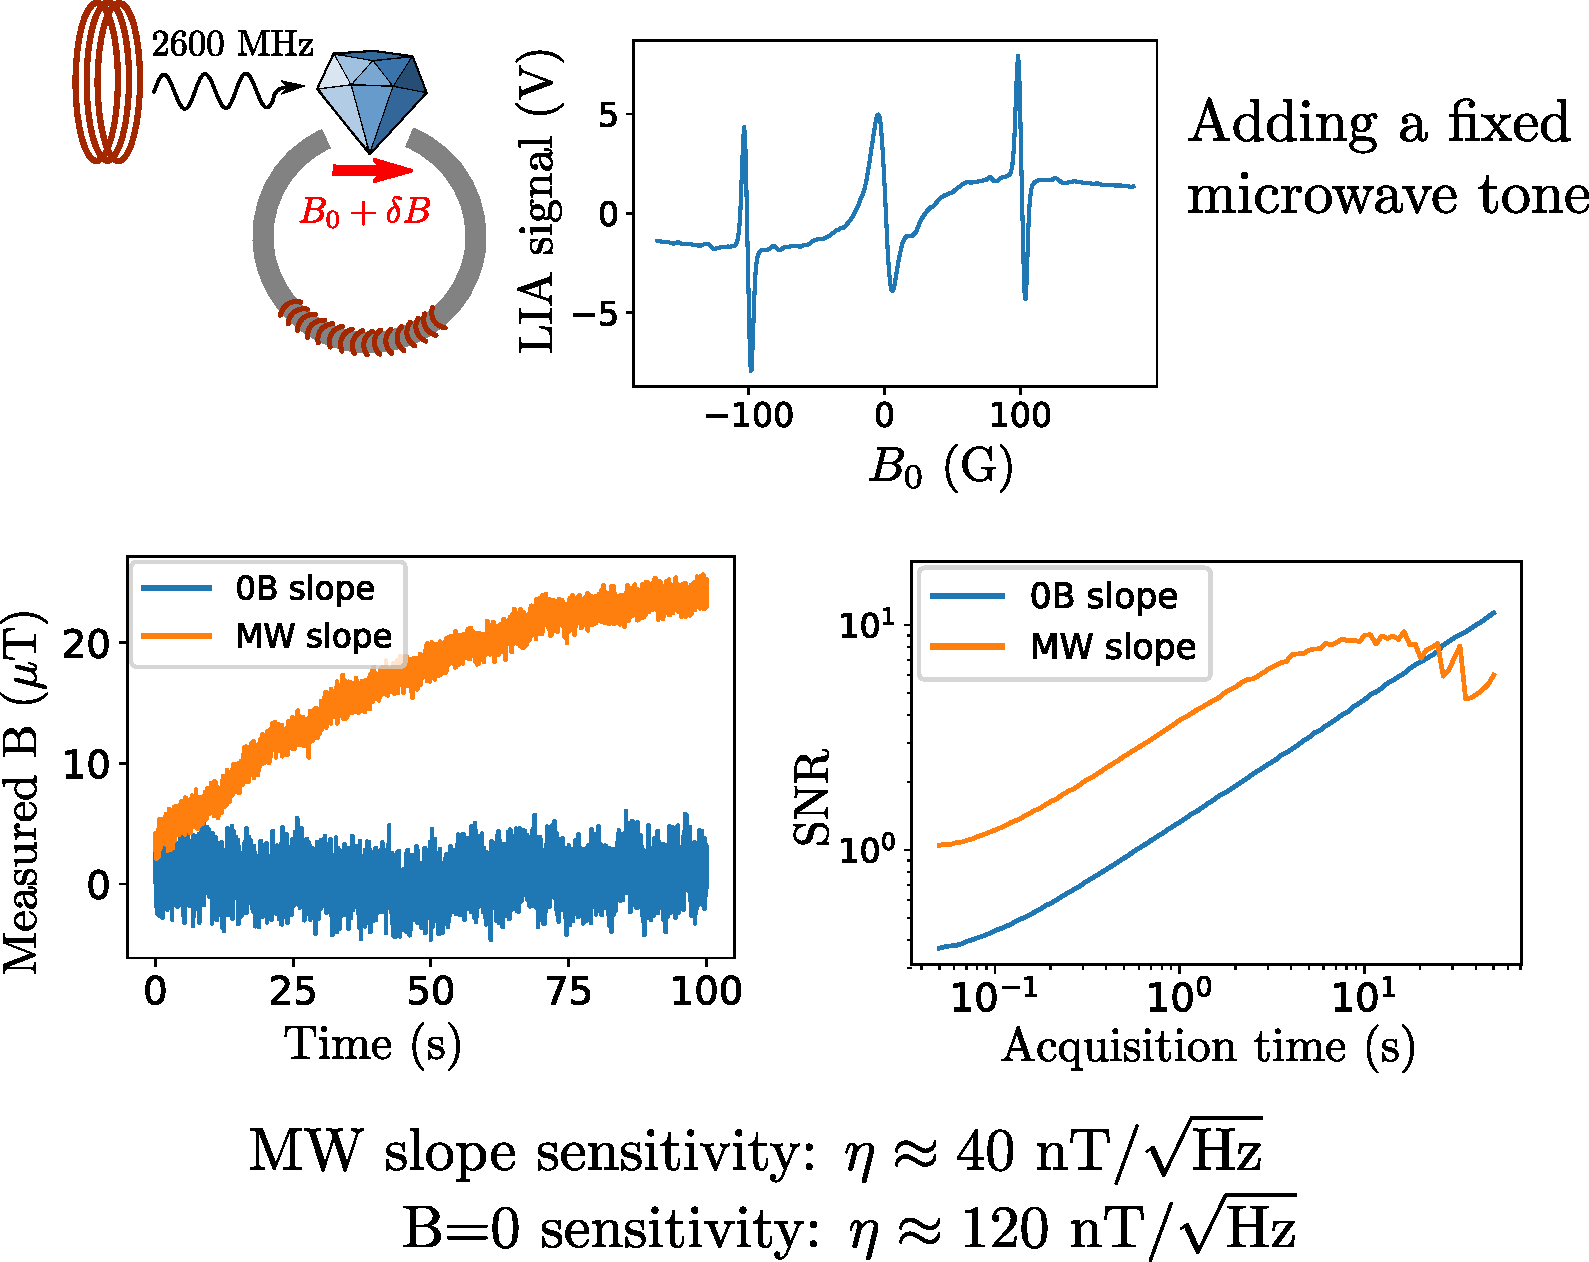
\includegraphics[width=\textwidth,height=0.9\textheight,keepaspectratio]{Slide_comparison_microwave}
\end{frame}

\begin{frame}{Angular sensitivity of LFDM}
\centering
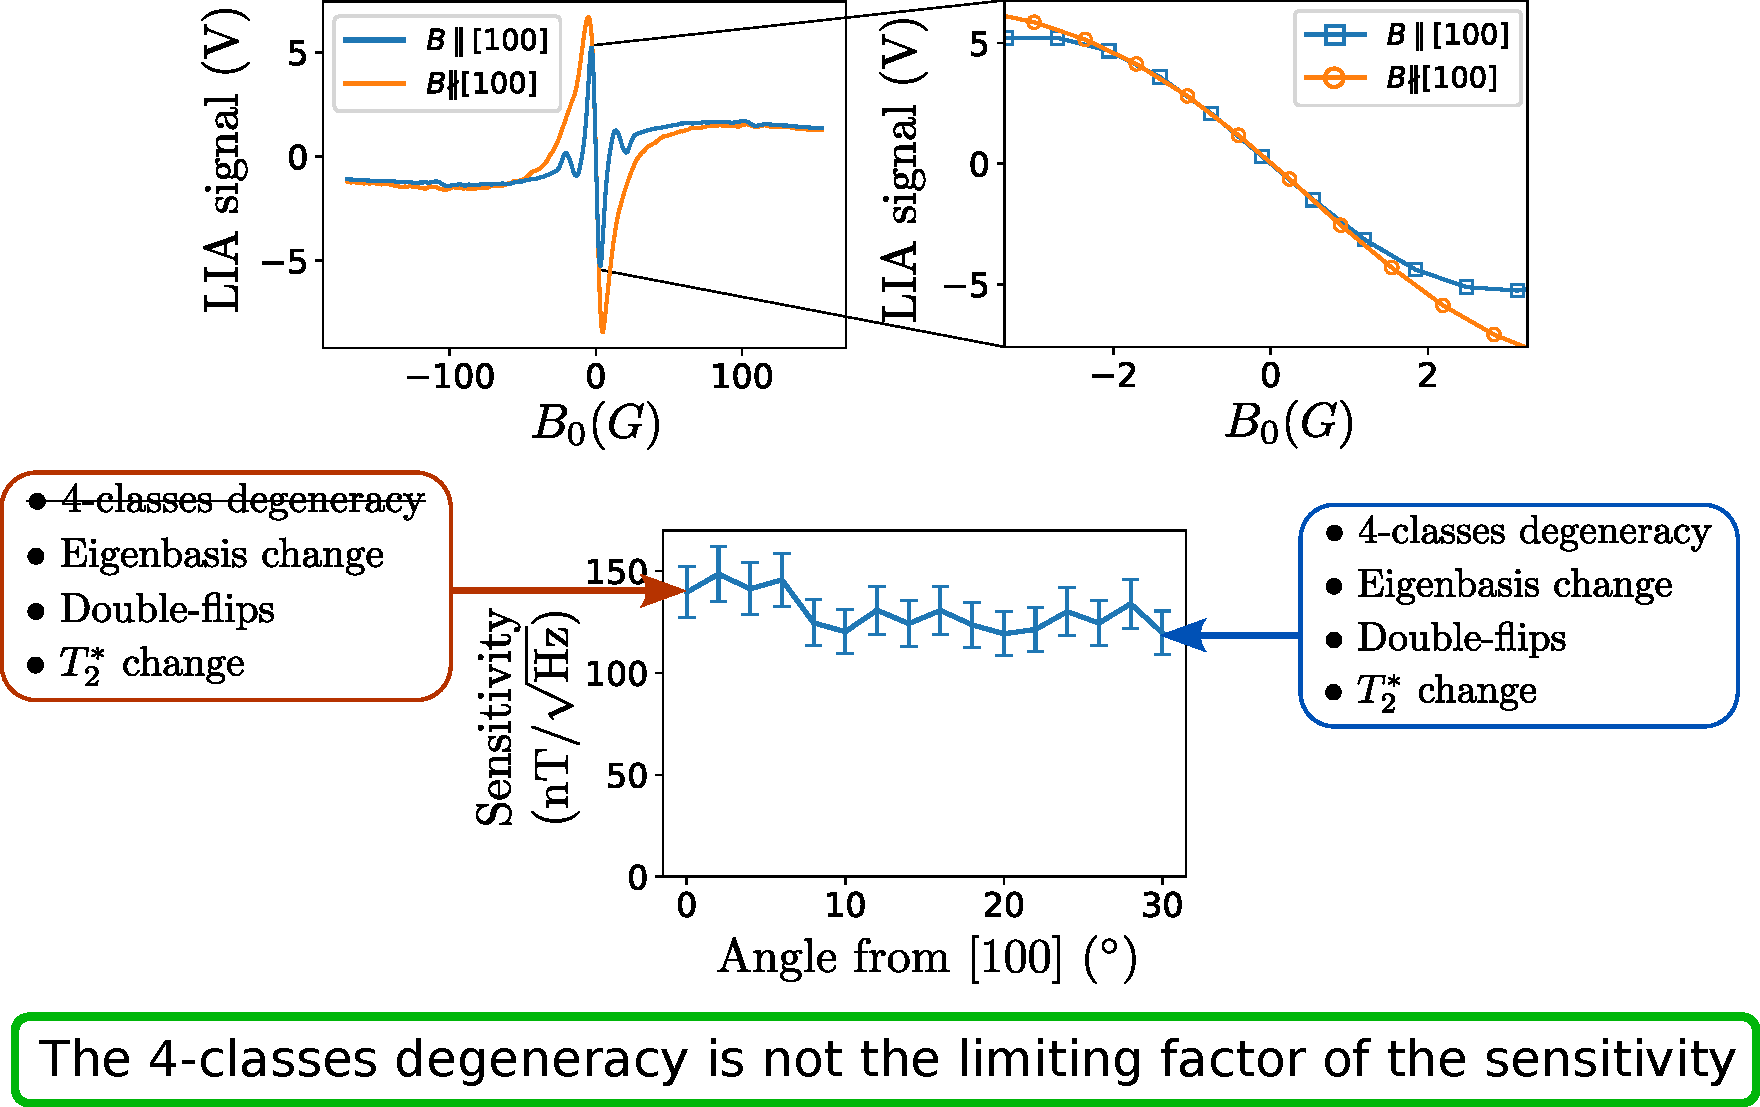
\includegraphics[width=\textwidth,height=0.9\textheight,keepaspectratio]{Slide_angular_sensitivity}
\end{frame}

\begin{frame}{Application: wide-field magnetometry on irregular surfaces}
\centering
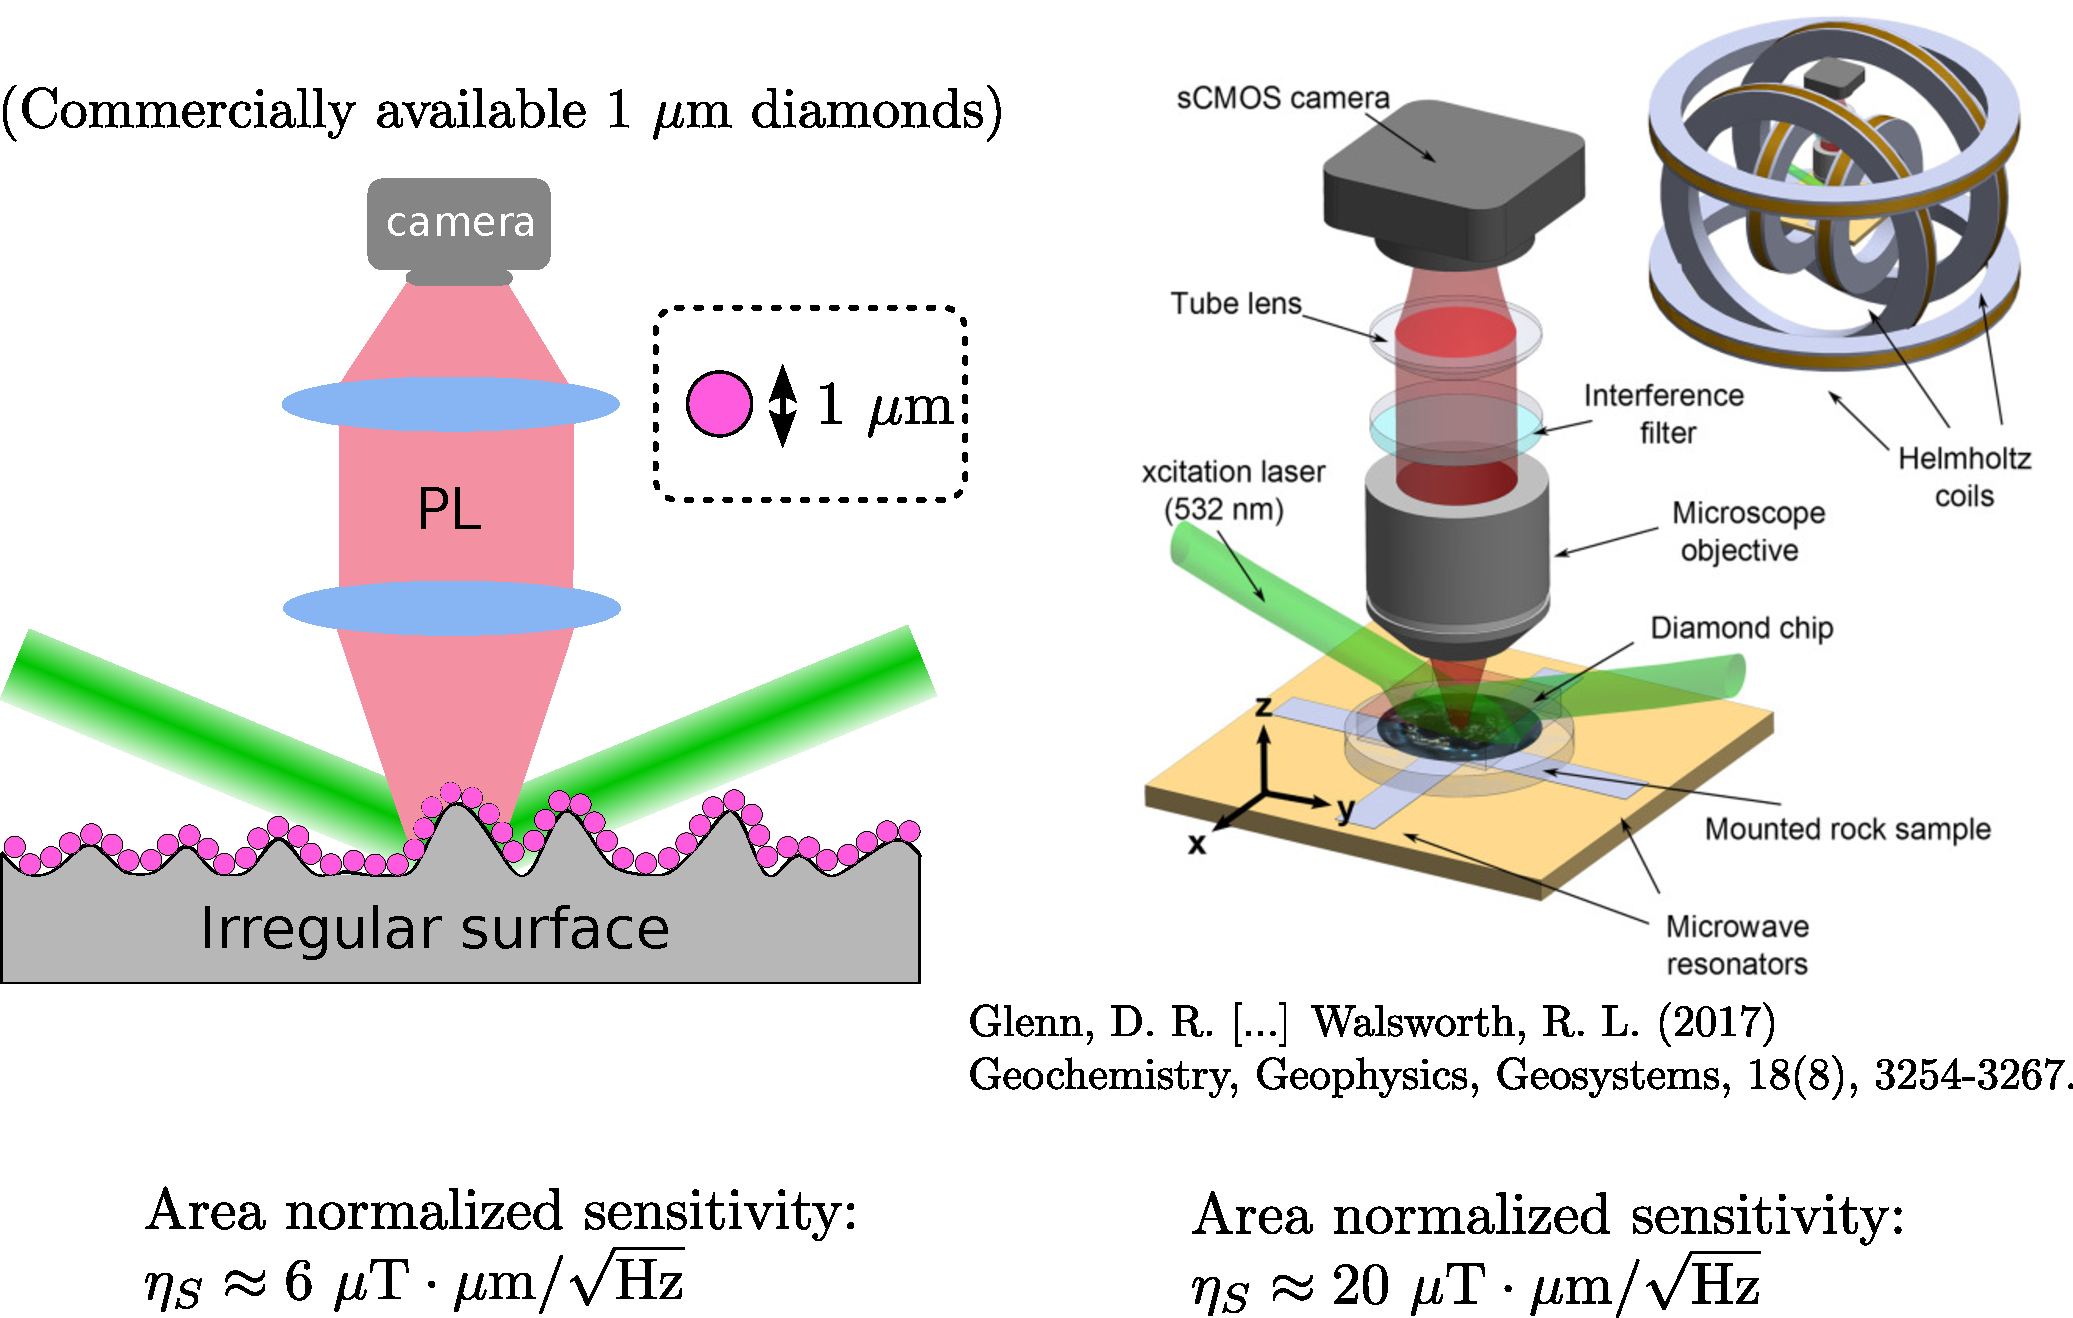
\includegraphics[width=\textwidth,height=0.9\textheight,keepaspectratio]{Slide_applications_wide_field}
\end{frame}

\begin{frame}{Other applications}
\centering
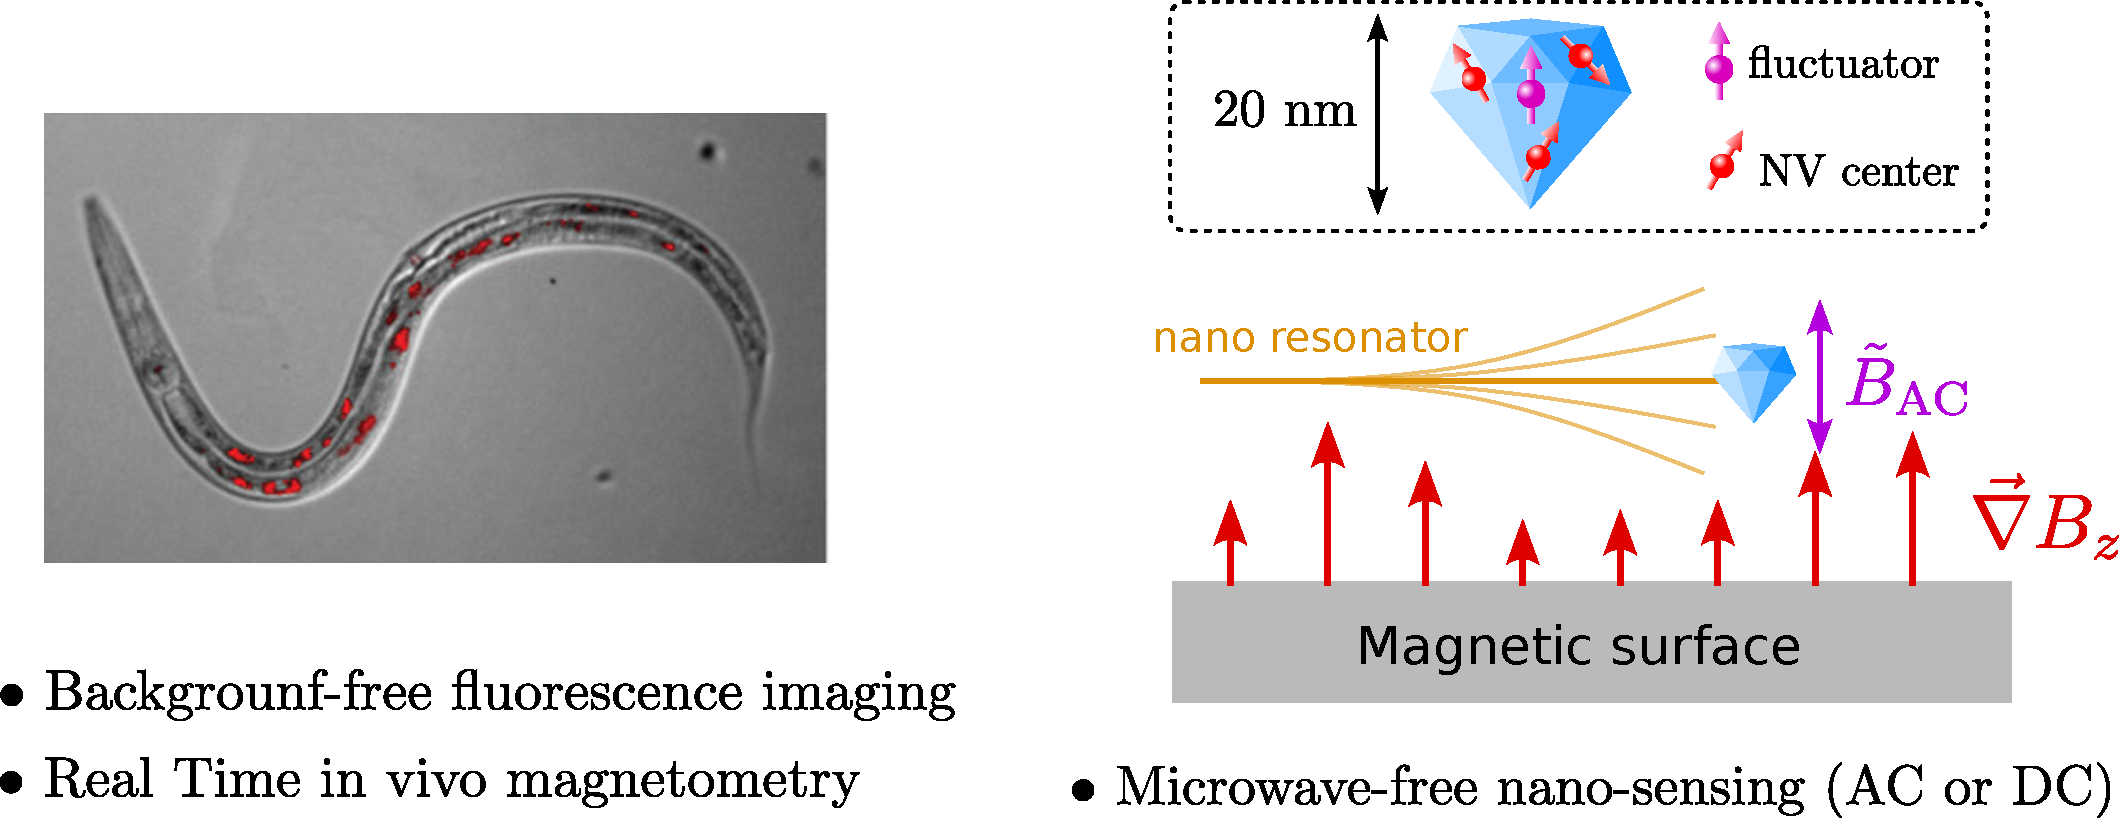
\includegraphics[width=\textwidth,height=0.9\textheight,keepaspectratio]{Slide_application_autre}
\end{frame}

\begin{frame}{Take home messages}
\begin{itemize}
\item The spin depolarization in dense NV ensemble is dominated by dipole-dipole interaction with fast decaying centers (fluctuators).
\medskip
\item The leading cause of depolarization in zero field is the spectral overlap of the NV classes, followed by the double flips.
\medskip
\item Low field depolarization magnetometry achieves a sensitivity $\sim 6\ \mu\rm T \cdot \mu \rm m^{3/2} / Hz^{1/2}$ with commercial samples.
\medskip
\item LFDM can be used with powder or polycristalline samples.
\end{itemize}

\end{frame}

\end{document}